\documentclass[12pt]{article}

\usepackage[brazil]{babel}
\usepackage[utf8]{inputenc}
\usepackage{lmodern}
\usepackage{graphicx}
\usepackage{float}
\usepackage{geometry}
\usepackage{setspace}
\usepackage{titlesec}

\geometry{a4paper, margin=2.5cm}

\titleformat{\section}
{\large\bfseries}
{\thesection}{1em}{}

\title{Análise Exploratória da Relação entre Consumo Energético e Emissões de CO$_2$ no Sistema Elétrico}
\author{S03-26 EQUIPE 44 - Data Science}
\date{\today}

\begin{document}

\onehalfspacing

\maketitle

\tableofcontents
\newpage

\section{Introdução}

A produção e o consumo de energia são fatores centrais para o desenvolvimento econômico, porém também representam uma das principais fontes de emissões de dióxido de carbono (CO$_2$). Compreender a relação entre matriz energética, consumo de energia e emissões é fundamental para avaliar impactos ambientais e orientar políticas energéticas.

Este relatório apresenta uma análise exploratória de dados (EDA) de um dataset que simula eventos de consumo energético associados a diferentes setores econômicos, regiões geográficas e fontes de geração elétrica.

O dataset utilizado neste estudo foi gerado de forma sintética com base em distribuições estatísticas e parâmetros inspirados em dados reais do sistema energético. Foram considerados fatores como fontes de geração elétrica, intensidade de carbono das tecnologias de geração, consumo energético por setor econômico, variação temporal ao longo do ano e distribuição geográfica por estados brasileiros.

Essa abordagem permite investigar padrões estruturais do sistema energético e explorar relações entre geração de energia e emissões de CO$_2$ de forma controlada.

\section{Estrutura da Matriz Energética}

\begin{figure}[H]
\centering
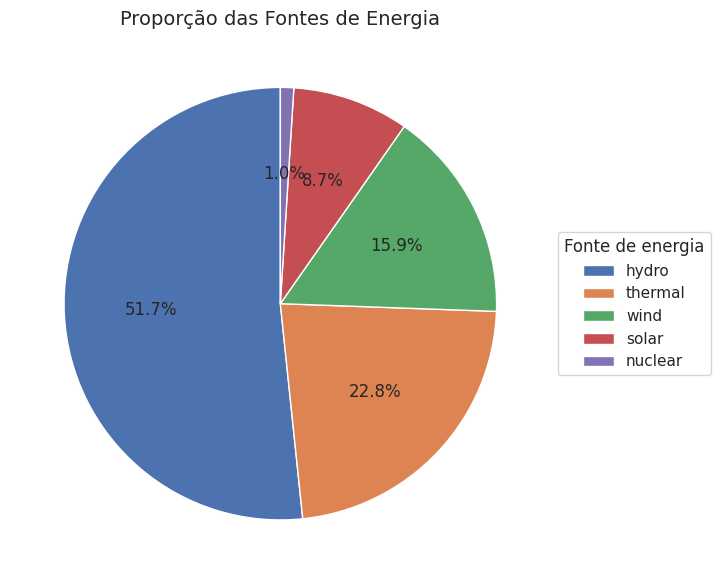
\includegraphics[width=0.8\textwidth]{images/Proporção_Fontes_Energia.png}
\caption{Distribuição das fontes de energia no dataset}
\end{figure}

Observa-se que a geração hidrelétrica representa a maior parcela da matriz energética, seguida pela geração térmica. Fontes renováveis como eólica e solar também possuem participação relevante.

\section{Consumo Médio de Energia por Setor}

\begin{figure}[H]
\centering
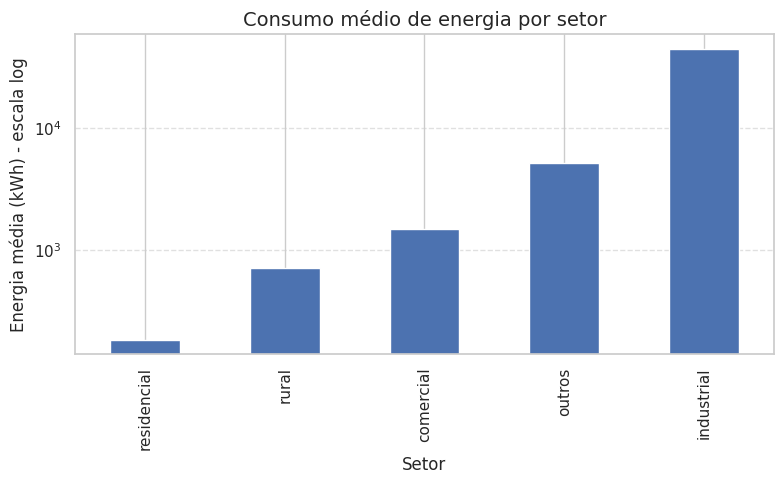
\includegraphics[width=0.8\textwidth]{images/Consume_medio_Setor.png}
\caption{Consumo médio de energia por setor}
\end{figure}

O setor industrial apresenta consumo energético significativamente superior aos demais setores, indicando forte dependência energética para atividades produtivas.

\section{Consumo Médio de Energia por Região}

\begin{figure}[H]
\centering
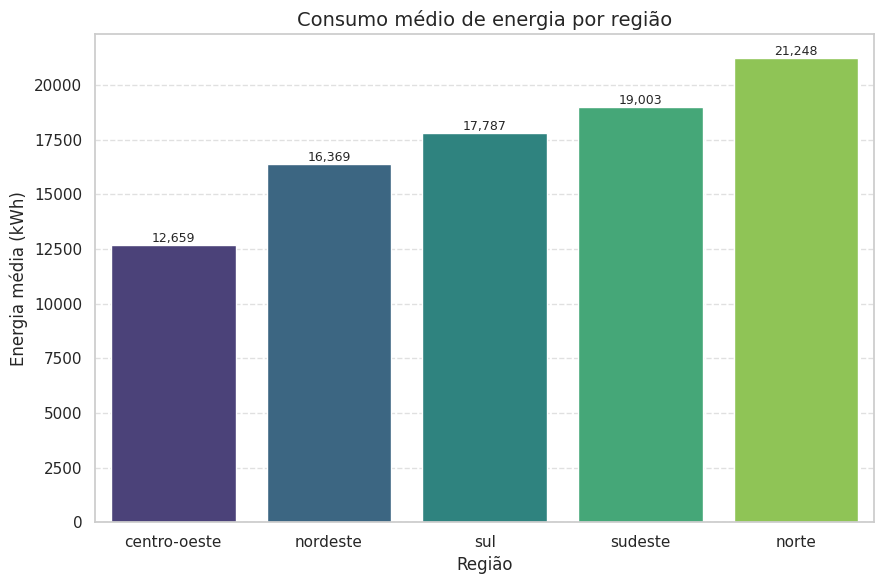
\includegraphics[width=0.8\textwidth]{images/Consumo médio de energia por região.png}
\caption{Consumo médio de energia por região}
\end{figure}

Diferenças regionais podem ser observadas, refletindo desigualdades na atividade econômica e na distribuição da infraestrutura energética.

\section{Intensidade de Carbono das Fontes Energéticas}

\begin{figure}[H]
\centering
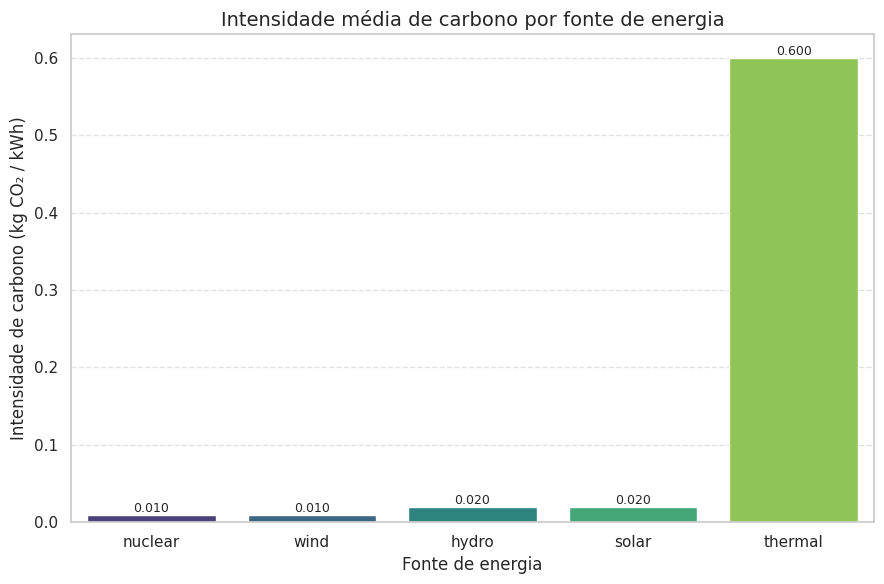
\includegraphics[width=0.8\textwidth]{images/Intensidade média de carbono por fonte de energia.png}
\caption{Intensidade média de carbono por fonte de energia}
\end{figure}

A geração térmica apresenta intensidade de carbono significativamente maior que as demais fontes, sendo responsável pela maior parte das emissões do sistema energético.

\section{Distribuição das Emissões de CO$_2$}

\begin{figure}[H]
\centering
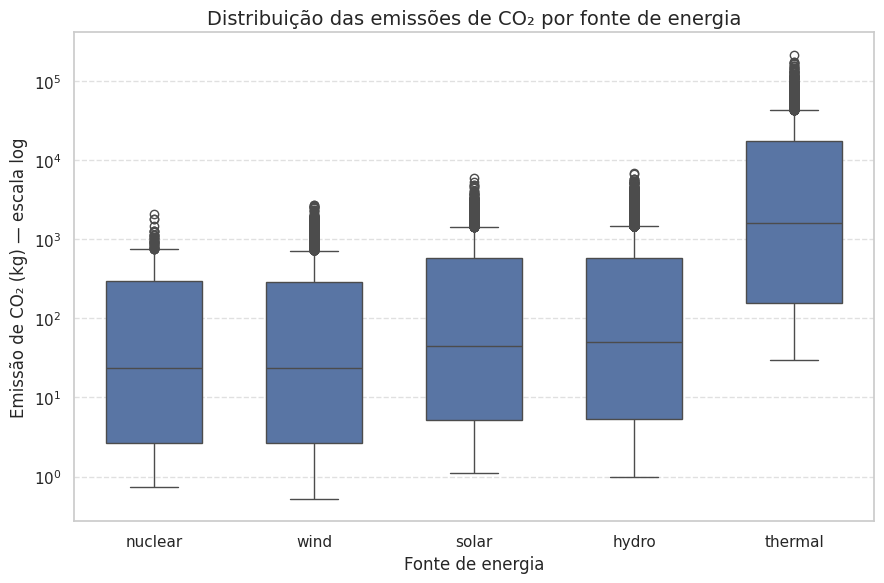
\includegraphics[width=0.8\textwidth]{images/Distribuição das emissões de CO₂ por fonte de energia.png}
\caption{Distribuição das emissões de CO$_2$ por fonte de energia}
\end{figure}

A distribuição das emissões evidencia a grande diferença entre fontes renováveis e fontes baseadas em combustíveis fósseis.

\section{Emissão Média de CO$_2$ por Fonte}

\begin{figure}[H]
\centering
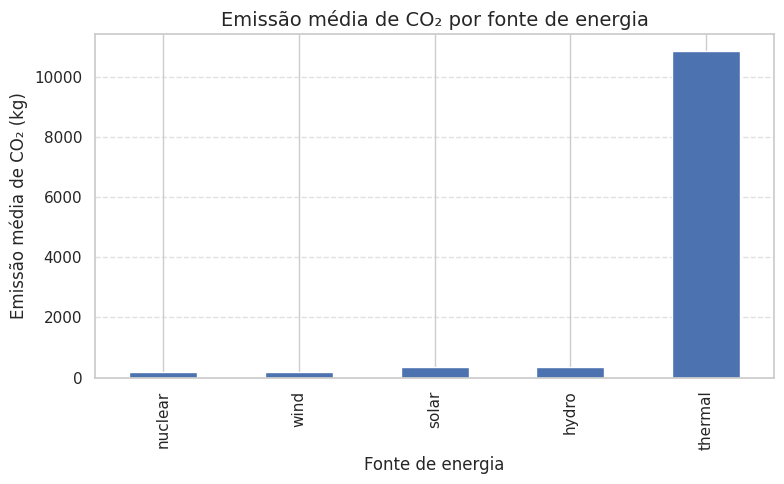
\includegraphics[width=0.8\textwidth]{images/Emissão média de CO₂ por fonte de energia.png}
\caption{Emissão média de CO$_2$ por fonte energética}
\end{figure}

Observa-se que fontes térmicas possuem emissões médias muito superiores às fontes renováveis.

\section{Emissão Total de CO$_2$ por Fonte}

\begin{figure}[H]
\centering
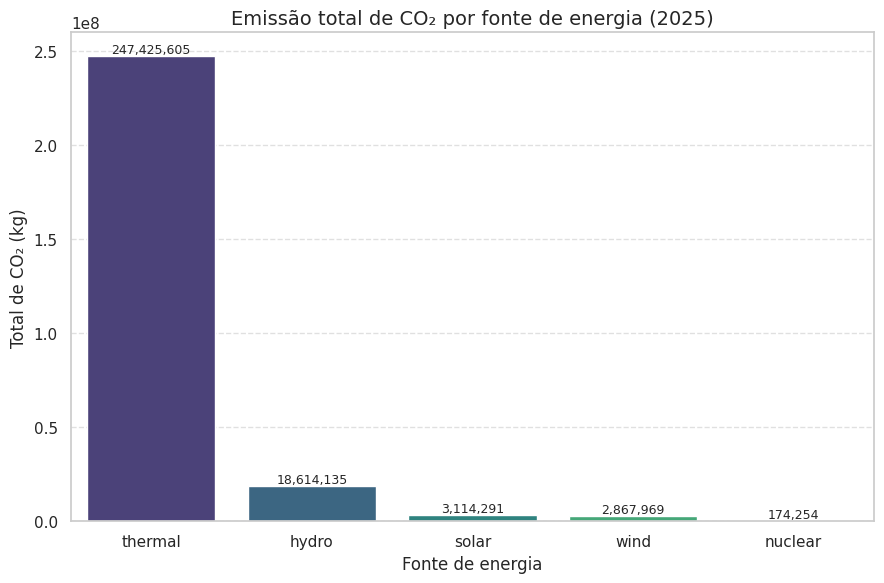
\includegraphics[width=0.8\textwidth]{images/Emissão total de CO₂ por fonte de energia (2025).png}
\caption{Emissão total de CO$_2$ por fonte de energia}
\end{figure}

A geração térmica domina as emissões totais devido à combinação de maior intensidade de carbono e participação relevante na geração energética.

\section{Distribuição de Intensidade de Carbono em Fontes de Baixa Emissão}

\begin{figure}[H]
\centering
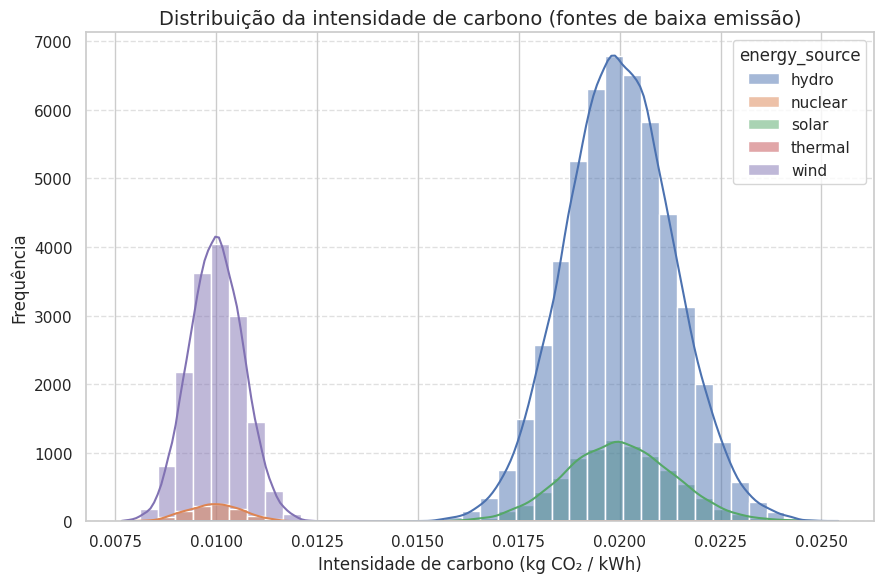
\includegraphics[width=0.8\textwidth]{images/Distribuição da intensidade de carbono (fontes de baixa emissão).png}
\caption{Distribuição da intensidade de carbono em fontes de baixa emissão}
\end{figure}

Fontes renováveis apresentam baixa intensidade de carbono e variação relativamente pequena entre si.

\section{Evolução Temporal das Emissões por Setor}

\begin{figure}[H]
\centering
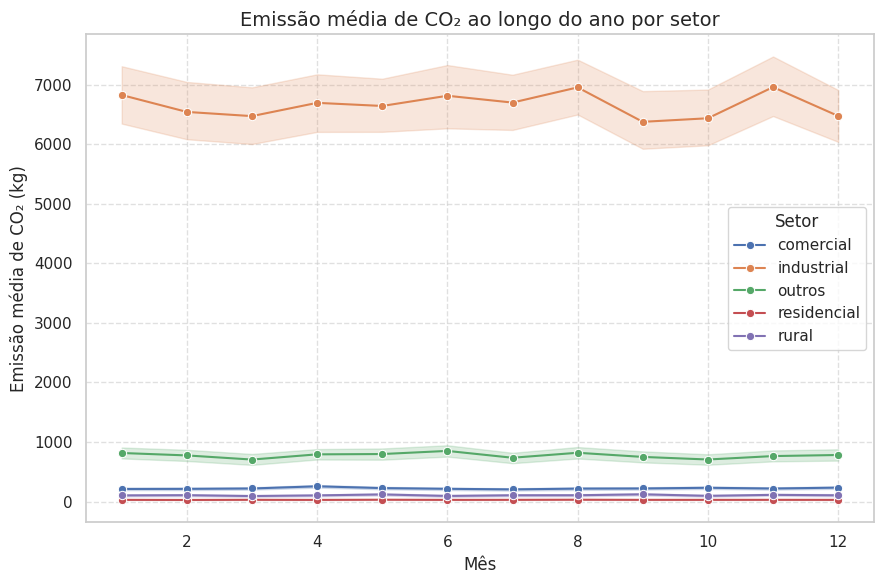
\includegraphics[width=0.9\textwidth]{images/Emissão média de CO₂ ao longo do ano por setor.png}
\caption{Emissão média de CO$_2$ ao longo do ano por setor}
\end{figure}

A análise temporal indica que o setor industrial mantém níveis de emissão consistentemente superiores aos demais.

\section{Distribuição Geográfica das Emissões}

\begin{figure}[H]
\centering
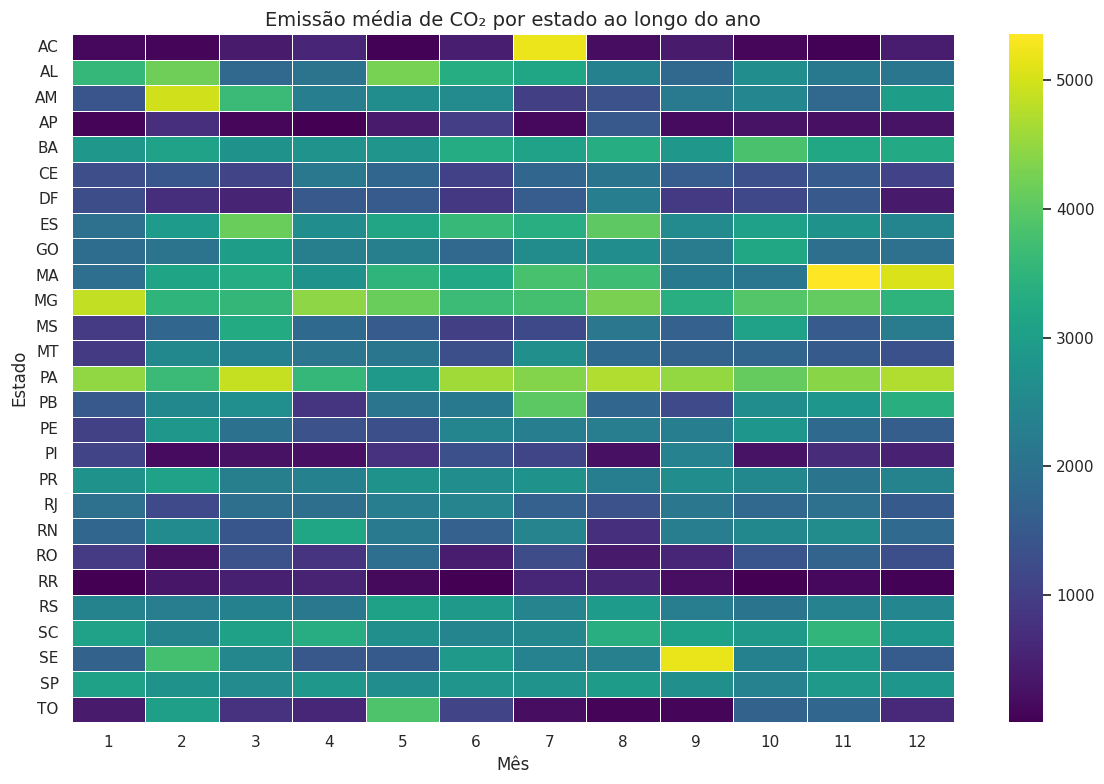
\includegraphics[width=0.9\textwidth]{images/Emissão média de CO₂ por estado ao longo do ano.png}
\caption{Emissão média de CO$_2$ por estado ao longo do ano}
\end{figure}

Diferenças regionais nas emissões podem estar associadas à distribuição da atividade econômica e à dependência de determinadas fontes energéticas.

\section{Participação da Geração Térmica}

\begin{figure}[H]
\centering
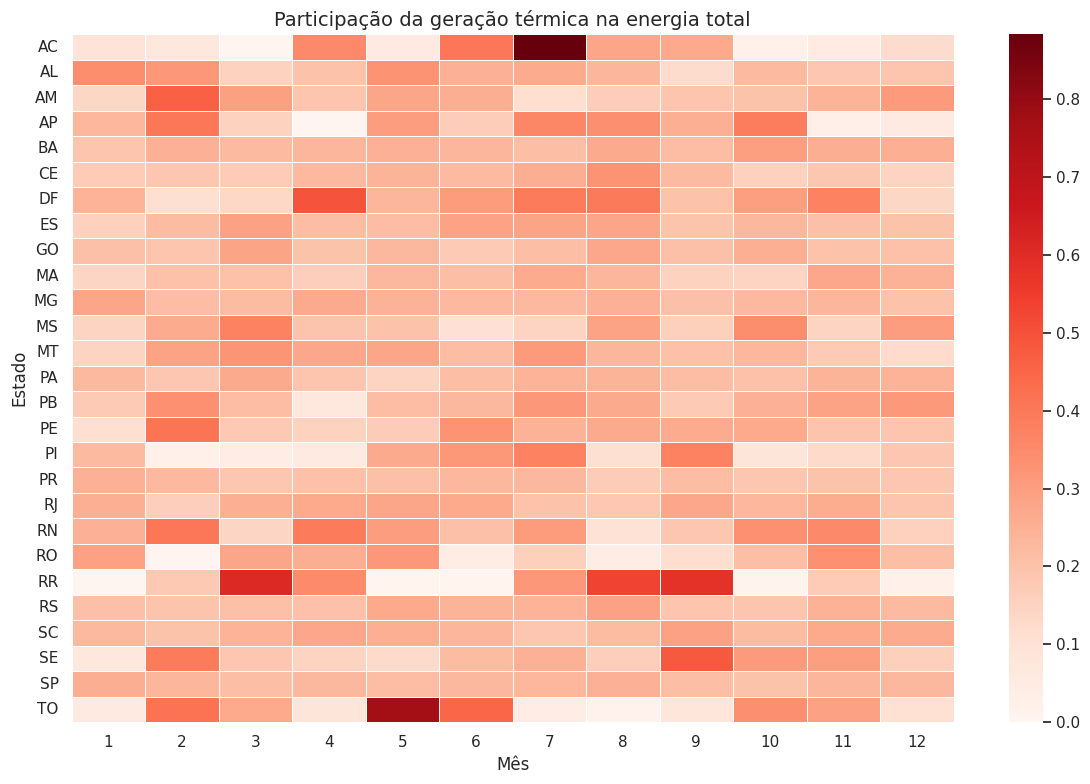
\includegraphics[width=0.9\textwidth]{images/Participação da geração térmica na energia total.png}
\caption{Participação da geração térmica ao longo do tempo}
\end{figure}

Algumas regiões apresentam maior dependência da geração térmica em determinados períodos.

\section{Relação entre Energia Gerada e Emissões}

\begin{figure}[H]
\centering
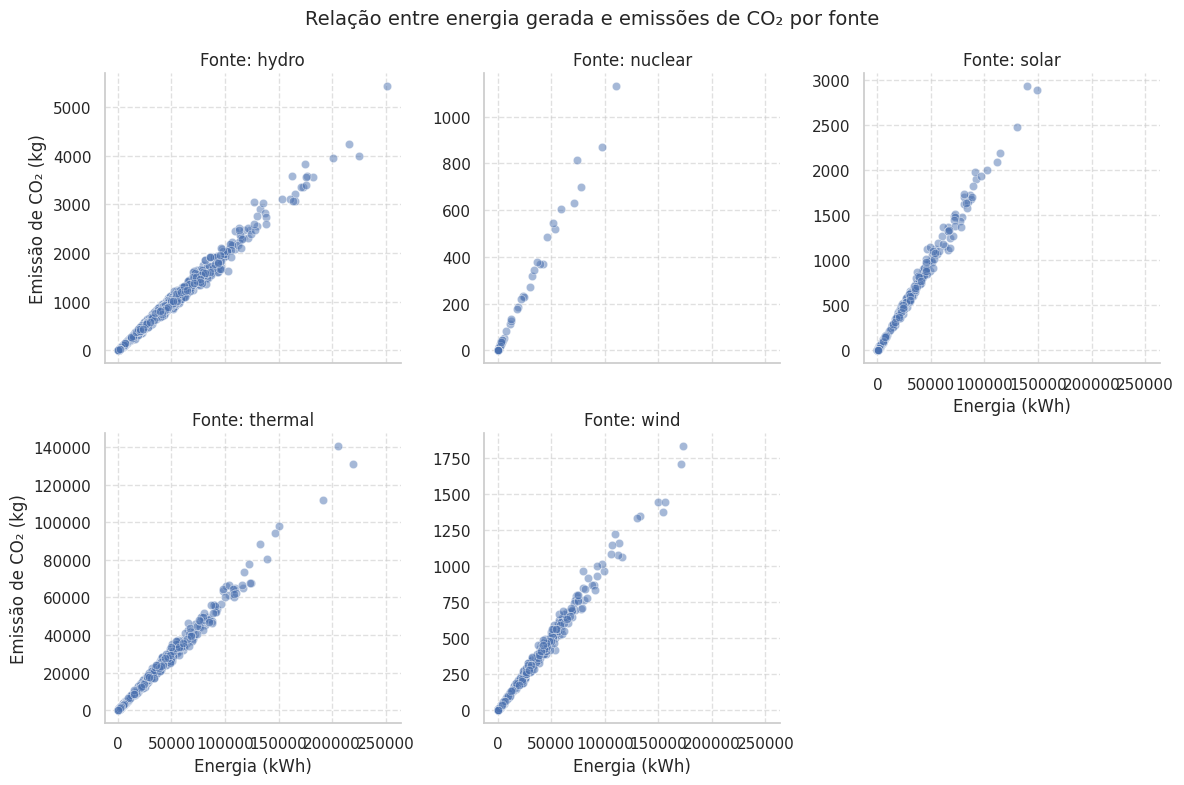
\includegraphics[width=0.9\textwidth]{images/Relação entre energia gerada e emissões de CO₂ por fonte.png}
\caption{Relação entre energia gerada e emissões de CO$_2$}
\end{figure}

Observa-se uma relação aproximadamente linear entre energia gerada e emissões, refletindo o modelo físico descrito pela seguinte equação:

\[
CO_2 = E \times I_c
\]

onde:

\begin{itemize}
\item $E$ representa a energia gerada em quilowatt-hora (kWh)
\item $I_c$ representa a intensidade de carbono da fonte energética (kg CO$_2$/kWh)
\end{itemize}

Essa relação evidencia que fontes com maior intensidade de carbono produzem maiores quantidades de emissões para o mesmo nível de geração energética.

\section{Conclusão}

A análise exploratória revelou padrões estruturais importantes no sistema energético simulado. O setor industrial concentra grande parte do consumo energético, enquanto a geração térmica é responsável pela maior parcela das emissões de CO$_2$.

Fontes renováveis como hidrelétrica, solar e eólica apresentam intensidade de carbono significativamente menor, reforçando seu papel na transição para sistemas energéticos de menor impacto ambiental.

Os resultados observados também confirmam o comportamento esperado do modelo físico de emissões, no qual as emissões totais são proporcionais à energia gerada e à intensidade de carbono da fonte energética.

O dataset apresenta comportamento consistente com sistemas energéticos reais e pode ser utilizado em etapas posteriores de modelagem, simulação e desenvolvimento de modelos preditivos relacionados à transição energética e redução de emissões.

\end{document}